%% fig_efoursix.tex   (generated by make_round45.py; do not edit by hand)
%% The diagonal at a lonely shift, interleaved shifts, and the arrangements within six values on E_0^8 (cor:efoursix).
\documentclass[tikz,border=8pt]{standalone}
\usepackage{amsmath,amssymb}
\usetikzlibrary{arrows.meta,calc,decorations.pathreplacing}
%% palette.tex -- shared colour definitions for the figures
\definecolor{PInk}{RGB}{26,32,44}
\definecolor{PBlue}{RGB}{37,82,139}
\definecolor{PTeal}{RGB}{23,127,125}
\definecolor{POchre}{RGB}{193,138,44}
\definecolor{PClay}{RGB}{178,74,58}
\definecolor{PSlate}{RGB}{108,122,137}
\definecolor{PViolet}{RGB}{110,86,150}
\definecolor{WBlue}{RGB}{223,234,246}
\definecolor{WTeal}{RGB}{220,238,236}
\definecolor{WOchre}{RGB}{250,240,218}
\definecolor{WClay}{RGB}{247,229,224}
\definecolor{WSlate}{RGB}{238,241,244}
\definecolor{PMag}{RGB}{158,58,110}
\definecolor{PGrass}{RGB}{62,124,66}
\definecolor{PAmber}{RGB}{214,112,38}
\definecolor{PIndigo}{RGB}{58,64,140}
\definecolor{PRule}{RGB}{176,186,197}

%% shared macros so the standalone figures match the paper
\providecommand{\QQ}{\mathbb{Q}}
\providecommand{\ZZ}{\mathbb{Z}}
\providecommand{\RR}{\mathbb{R}}
\providecommand{\CC}{\mathbb{C}}
\providecommand{\PP}{\mathbb{P}}
\providecommand{\Kx}{K^{\times}}
\providecommand{\HW}{W}
\providecommand{\Nm}{\mathrm{N}}
\providecommand{\Hdg}{\mathrm{Hdg}}
\providecommand{\NS}{\mathrm{NS}}
\providecommand{\cA}{\mathcal{A}}
\providecommand{\cD}{\mathcal{D}}
\providecommand{\cF}{\mathcal{F}}
\providecommand{\cP}{\mathcal{P}}
\providecommand{\cO}{\mathcal{O}}
\providecommand{\cQ}{\mathcal{Q}}
\providecommand{\bbar}[1]{\overline{#1}}
\providecommand{\ch}{\operatorname{ch}}
\providecommand{\End}{\mathrm{End}}
\providecommand{\Ext}{\operatorname{Ext}}
\providecommand{\Supp}{\operatorname{Supp}}

\begin{document}
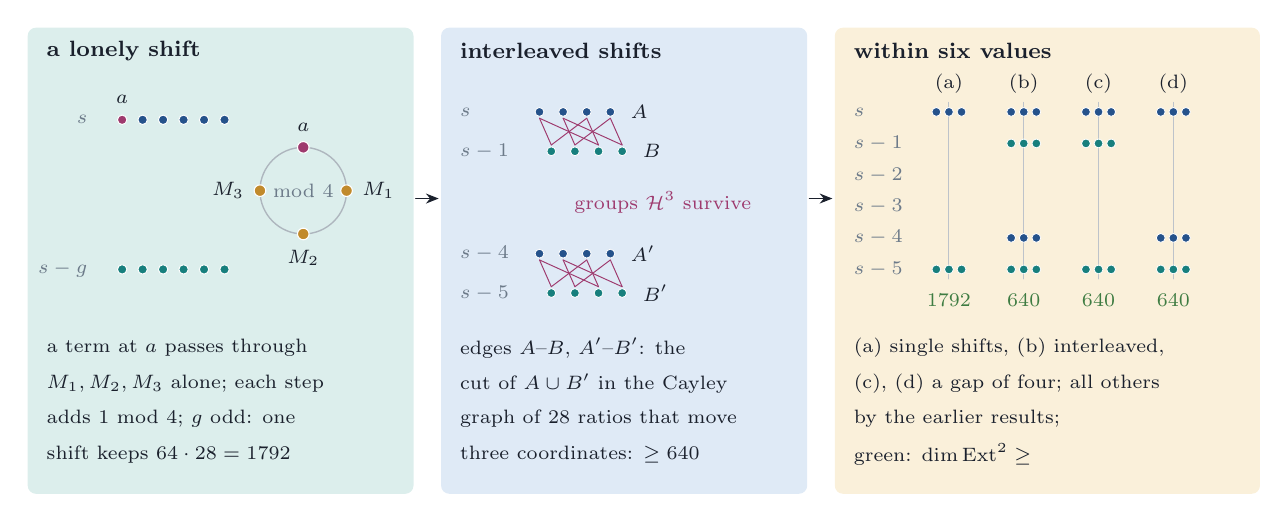
\begin{tikzpicture}[x=1cm,y=1cm,line join=round,line cap=round,
  font=\small,text=PInk,lbl/.style={inner sep=1pt}]
  \path[fill=WTeal,draw=none,rounded corners=3.0pt] (0.0500,-1.3000) rectangle (4.9500,4.6200);
  \draw[PSlate!55!white,line width=0.50pt] (3.5500,2.5500) circle (0.5500);
  \path[fill=WBlue,draw=none,rounded corners=3.0pt] (5.3000,-1.3000) rectangle (9.9500,4.6200);
  \path[fill=WOchre,draw=none,rounded corners=3.0pt] (10.3000,-1.3000) rectangle (15.7000,4.6200);
  \path[fill=PMag,draw=white,line width=0.35pt] (1.2500,3.4500) circle (1.70pt);
  \path[fill=PTeal,draw=white,line width=0.35pt] (1.2500,1.5500) circle (1.70pt);
  \path[fill=PBlue,draw=white,line width=0.35pt] (1.5100,3.4500) circle (1.70pt);
  \path[fill=PTeal,draw=white,line width=0.35pt] (1.5100,1.5500) circle (1.70pt);
  \path[fill=PBlue,draw=white,line width=0.35pt] (1.7700,3.4500) circle (1.70pt);
  \path[fill=PTeal,draw=white,line width=0.35pt] (1.7700,1.5500) circle (1.70pt);
  \path[fill=PBlue,draw=white,line width=0.35pt] (2.0300,3.4500) circle (1.70pt);
  \path[fill=PTeal,draw=white,line width=0.35pt] (2.0300,1.5500) circle (1.70pt);
  \path[fill=PBlue,draw=white,line width=0.35pt] (2.2900,3.4500) circle (1.70pt);
  \path[fill=PTeal,draw=white,line width=0.35pt] (2.2900,1.5500) circle (1.70pt);
  \path[fill=PBlue,draw=white,line width=0.35pt] (2.5500,3.4500) circle (1.70pt);
  \path[fill=PTeal,draw=white,line width=0.35pt] (2.5500,1.5500) circle (1.70pt);
  \path[fill=PMag,draw=white,line width=0.40pt] (3.5500,3.1000) circle (2.10pt);
  \path[fill=POchre,draw=white,line width=0.40pt] (4.1000,2.5500) circle (2.10pt);
  \path[fill=POchre,draw=white,line width=0.40pt] (3.5500,2.0000) circle (2.10pt);
  \path[fill=POchre,draw=white,line width=0.40pt] (3.0000,2.5500) circle (2.10pt);
  \draw[PMag,line width=0.35pt] (6.5500,3.4700) -- (6.7000,3.1300);
  \draw[PMag,line width=0.35pt] (6.5500,3.4700) -- (7.3000,3.1300);
  \draw[PMag,line width=0.35pt] (6.8500,3.4700) -- (7.0000,3.1300);
  \draw[PMag,line width=0.35pt] (6.8500,3.4700) -- (7.6000,3.1300);
  \draw[PMag,line width=0.35pt] (7.1500,3.4700) -- (6.7000,3.1300);
  \draw[PMag,line width=0.35pt] (7.1500,3.4700) -- (7.3000,3.1300);
  \draw[PMag,line width=0.35pt] (7.4500,3.4700) -- (7.0000,3.1300);
  \draw[PMag,line width=0.35pt] (7.4500,3.4700) -- (7.6000,3.1300);
  \draw[PMag,line width=0.35pt] (6.5500,1.6700) -- (6.7000,1.3300);
  \draw[PMag,line width=0.35pt] (6.5500,1.6700) -- (7.3000,1.3300);
  \draw[PMag,line width=0.35pt] (6.8500,1.6700) -- (7.0000,1.3300);
  \draw[PMag,line width=0.35pt] (6.8500,1.6700) -- (7.6000,1.3300);
  \draw[PMag,line width=0.35pt] (7.1500,1.6700) -- (6.7000,1.3300);
  \draw[PMag,line width=0.35pt] (7.1500,1.6700) -- (7.3000,1.3300);
  \draw[PMag,line width=0.35pt] (7.4500,1.6700) -- (7.0000,1.3300);
  \draw[PMag,line width=0.35pt] (7.4500,1.6700) -- (7.6000,1.3300);
  \path[fill=PBlue,draw=white,line width=0.30pt] (6.5500,3.5500) circle (1.60pt);
  \path[fill=PBlue,draw=white,line width=0.30pt] (6.8500,3.5500) circle (1.60pt);
  \path[fill=PBlue,draw=white,line width=0.30pt] (7.1500,3.5500) circle (1.60pt);
  \path[fill=PBlue,draw=white,line width=0.30pt] (7.4500,3.5500) circle (1.60pt);
  \path[fill=PTeal,draw=white,line width=0.30pt] (6.7000,3.0500) circle (1.60pt);
  \path[fill=PTeal,draw=white,line width=0.30pt] (7.0000,3.0500) circle (1.60pt);
  \path[fill=PTeal,draw=white,line width=0.30pt] (7.3000,3.0500) circle (1.60pt);
  \path[fill=PTeal,draw=white,line width=0.30pt] (7.6000,3.0500) circle (1.60pt);
  \path[fill=PBlue,draw=white,line width=0.30pt] (6.5500,1.7500) circle (1.60pt);
  \path[fill=PBlue,draw=white,line width=0.30pt] (6.8500,1.7500) circle (1.60pt);
  \path[fill=PBlue,draw=white,line width=0.30pt] (7.1500,1.7500) circle (1.60pt);
  \path[fill=PBlue,draw=white,line width=0.30pt] (7.4500,1.7500) circle (1.60pt);
  \path[fill=PTeal,draw=white,line width=0.30pt] (6.7000,1.2500) circle (1.60pt);
  \path[fill=PTeal,draw=white,line width=0.30pt] (7.0000,1.2500) circle (1.60pt);
  \path[fill=PTeal,draw=white,line width=0.30pt] (7.3000,1.2500) circle (1.60pt);
  \path[fill=PTeal,draw=white,line width=0.30pt] (7.6000,1.2500) circle (1.60pt);
  \draw[PSlate!45!white,line width=0.4pt] (11.7500,3.6700) -- (11.7500,1.4300);
  \path[fill=PBlue,draw=white,line width=0.30pt] (11.5900,3.5500) circle (1.60pt);
  \path[fill=PBlue,draw=white,line width=0.30pt] (11.7500,3.5500) circle (1.60pt);
  \path[fill=PBlue,draw=white,line width=0.30pt] (11.9100,3.5500) circle (1.60pt);
  \path[fill=PTeal,draw=white,line width=0.30pt] (11.5900,1.5500) circle (1.60pt);
  \path[fill=PTeal,draw=white,line width=0.30pt] (11.7500,1.5500) circle (1.60pt);
  \path[fill=PTeal,draw=white,line width=0.30pt] (11.9100,1.5500) circle (1.60pt);
  \draw[PSlate!45!white,line width=0.4pt] (12.7000,3.6700) -- (12.7000,1.4300);
  \path[fill=PBlue,draw=white,line width=0.30pt] (12.5400,3.5500) circle (1.60pt);
  \path[fill=PBlue,draw=white,line width=0.30pt] (12.7000,3.5500) circle (1.60pt);
  \path[fill=PBlue,draw=white,line width=0.30pt] (12.8600,3.5500) circle (1.60pt);
  \path[fill=PBlue,draw=white,line width=0.30pt] (12.5400,1.9500) circle (1.60pt);
  \path[fill=PBlue,draw=white,line width=0.30pt] (12.7000,1.9500) circle (1.60pt);
  \path[fill=PBlue,draw=white,line width=0.30pt] (12.8600,1.9500) circle (1.60pt);
  \path[fill=PTeal,draw=white,line width=0.30pt] (12.5400,3.1500) circle (1.60pt);
  \path[fill=PTeal,draw=white,line width=0.30pt] (12.7000,3.1500) circle (1.60pt);
  \path[fill=PTeal,draw=white,line width=0.30pt] (12.8600,3.1500) circle (1.60pt);
  \path[fill=PTeal,draw=white,line width=0.30pt] (12.5400,1.5500) circle (1.60pt);
  \path[fill=PTeal,draw=white,line width=0.30pt] (12.7000,1.5500) circle (1.60pt);
  \path[fill=PTeal,draw=white,line width=0.30pt] (12.8600,1.5500) circle (1.60pt);
  \draw[PSlate!45!white,line width=0.4pt] (13.6500,3.6700) -- (13.6500,1.4300);
  \path[fill=PBlue,draw=white,line width=0.30pt] (13.4900,3.5500) circle (1.60pt);
  \path[fill=PBlue,draw=white,line width=0.30pt] (13.6500,3.5500) circle (1.60pt);
  \path[fill=PBlue,draw=white,line width=0.30pt] (13.8100,3.5500) circle (1.60pt);
  \path[fill=PTeal,draw=white,line width=0.30pt] (13.4900,3.1500) circle (1.60pt);
  \path[fill=PTeal,draw=white,line width=0.30pt] (13.6500,3.1500) circle (1.60pt);
  \path[fill=PTeal,draw=white,line width=0.30pt] (13.8100,3.1500) circle (1.60pt);
  \path[fill=PTeal,draw=white,line width=0.30pt] (13.4900,1.5500) circle (1.60pt);
  \path[fill=PTeal,draw=white,line width=0.30pt] (13.6500,1.5500) circle (1.60pt);
  \path[fill=PTeal,draw=white,line width=0.30pt] (13.8100,1.5500) circle (1.60pt);
  \draw[PSlate!45!white,line width=0.4pt] (14.6000,3.6700) -- (14.6000,1.4300);
  \path[fill=PBlue,draw=white,line width=0.30pt] (14.4400,3.5500) circle (1.60pt);
  \path[fill=PBlue,draw=white,line width=0.30pt] (14.6000,3.5500) circle (1.60pt);
  \path[fill=PBlue,draw=white,line width=0.30pt] (14.7600,3.5500) circle (1.60pt);
  \path[fill=PBlue,draw=white,line width=0.30pt] (14.4400,1.9500) circle (1.60pt);
  \path[fill=PBlue,draw=white,line width=0.30pt] (14.6000,1.9500) circle (1.60pt);
  \path[fill=PBlue,draw=white,line width=0.30pt] (14.7600,1.9500) circle (1.60pt);
  \path[fill=PTeal,draw=white,line width=0.30pt] (14.4400,1.5500) circle (1.60pt);
  \path[fill=PTeal,draw=white,line width=0.30pt] (14.6000,1.5500) circle (1.60pt);
  \path[fill=PTeal,draw=white,line width=0.30pt] (14.7600,1.5500) circle (1.60pt);
  \draw[PInk,line width=0.6pt,-{Stealth[length=4.6pt,width=3.6pt]}] (4.9800,2.4500) -- (5.2700,2.4500);
  \draw[PInk,line width=0.6pt,-{Stealth[length=4.6pt,width=3.6pt]}] (9.9800,2.4500) -- (10.2700,2.4500);
  \node[lbl,anchor=west,text=PInk,font=\footnotesize] at (0.2500,4.3200) {\textbf{a lonely shift}};
  \node[lbl,anchor=east,text=PSlate,font=\scriptsize] at (0.8500,3.4500) {$s$};
  \node[lbl,anchor=east,text=PSlate,font=\scriptsize] at (0.8500,1.5500) {$s-g$};
  \node[lbl,anchor=south,text=PInk,font=\scriptsize] at (1.2500,3.6100) {$a$};
  \node[lbl,anchor=south,text=PInk,font=\scriptsize] at (3.5500,3.2600) {$a$};
  \node[lbl,anchor=west,text=PInk,font=\scriptsize] at (4.2600,2.5500) {$M_{1}$};
  \node[lbl,anchor=north,text=PInk,font=\scriptsize] at (3.5500,1.8400) {$M_{2}$};
  \node[lbl,anchor=east,text=PInk,font=\scriptsize] at (2.8400,2.5500) {$M_{3}$};
  \node[lbl,text=PSlate,font=\scriptsize] at (3.5500,2.5500) {mod $4$};
  \node[lbl,anchor=west,text=PInk,font=\scriptsize] at (0.2500,0.5500) {a term at $a$ passes through};
  \node[lbl,anchor=west,text=PInk,font=\scriptsize] at (0.2500,0.1000) {$M_{1},M_{2},M_{3}$ alone; each step};
  \node[lbl,anchor=west,text=PInk,font=\scriptsize] at (0.2500,-0.3500) {adds $1$ mod $4$; $g$ odd: one};
  \node[lbl,anchor=west,text=PInk,font=\scriptsize] at (0.2500,-0.8000) {shift keeps $64\cdot28=1792$};
  \node[lbl,anchor=west,text=PInk,font=\footnotesize] at (5.5000,4.3200) {\textbf{interleaved shifts}};
  \node[lbl,anchor=west,text=PSlate,font=\scriptsize] at (5.5000,3.5500) {$s$};
  \node[lbl,anchor=west,text=PSlate,font=\scriptsize] at (5.5000,3.0500) {$s-1$};
  \node[lbl,anchor=west,text=PSlate,font=\scriptsize] at (5.5000,1.7500) {$s-4$};
  \node[lbl,anchor=west,text=PSlate,font=\scriptsize] at (5.5000,1.2500) {$s-5$};
  \node[lbl,anchor=west,text=PInk,font=\scriptsize] at (7.6700,3.5500) {$A$};
  \node[lbl,anchor=west,text=PInk,font=\scriptsize] at (7.8200,3.0500) {$B$};
  \node[lbl,anchor=west,text=PInk,font=\scriptsize] at (7.6700,1.7500) {$A'$};
  \node[lbl,anchor=west,text=PInk,font=\scriptsize] at (7.8200,1.2500) {$B'$};
  \node[lbl,anchor=west,text=PMag,font=\scriptsize] at (6.9500,2.4000) {groups $\mathcal{H}^{3}$ survive};
  \node[lbl,anchor=west,text=PInk,font=\scriptsize] at (5.5000,0.5500) {edges $A$--$B$, $A'$--$B'$: the};
  \node[lbl,anchor=west,text=PInk,font=\scriptsize] at (5.5000,0.1000) {cut of $A\cup B'$ in the Cayley};
  \node[lbl,anchor=west,text=PInk,font=\scriptsize] at (5.5000,-0.3500) {graph of $28$ ratios that move};
  \node[lbl,anchor=west,text=PInk,font=\scriptsize] at (5.5000,-0.8000) {three coordinates: $\ge640$};
  \node[lbl,anchor=west,text=PInk,font=\footnotesize] at (10.5000,4.3200) {\textbf{within six values}};
  \node[lbl,anchor=west,text=PSlate,font=\scriptsize] at (10.5000,3.5500) {$s$};
  \node[lbl,anchor=west,text=PSlate,font=\scriptsize] at (10.5000,3.1500) {$s-1$};
  \node[lbl,anchor=west,text=PSlate,font=\scriptsize] at (10.5000,2.7500) {$s-2$};
  \node[lbl,anchor=west,text=PSlate,font=\scriptsize] at (10.5000,2.3500) {$s-3$};
  \node[lbl,anchor=west,text=PSlate,font=\scriptsize] at (10.5000,1.9500) {$s-4$};
  \node[lbl,anchor=west,text=PSlate,font=\scriptsize] at (10.5000,1.5500) {$s-5$};
  \node[lbl,anchor=south,text=PInk,font=\scriptsize] at (11.7500,3.7500) {(a)};
  \node[lbl,anchor=south,text=PInk,font=\scriptsize] at (12.7000,3.7500) {(b)};
  \node[lbl,anchor=south,text=PInk,font=\scriptsize] at (13.6500,3.7500) {(c)};
  \node[lbl,anchor=south,text=PInk,font=\scriptsize] at (14.6000,3.7500) {(d)};
  \node[lbl,anchor=north,text=PGrass,font=\scriptsize] at (11.7500,1.2800) {$1792$};
  \node[lbl,anchor=north,text=PGrass,font=\scriptsize] at (12.7000,1.2800) {$640$};
  \node[lbl,anchor=north,text=PGrass,font=\scriptsize] at (13.6500,1.2800) {$640$};
  \node[lbl,anchor=north,text=PGrass,font=\scriptsize] at (14.6000,1.2800) {$640$};
  \node[lbl,anchor=west,text=PInk,font=\scriptsize] at (10.5000,0.5500) {(a) single shifts, (b) interleaved,};
  \node[lbl,anchor=west,text=PInk,font=\scriptsize] at (10.5000,0.1000) {(c), (d) a gap of four; all others};
  \node[lbl,anchor=west,text=PInk,font=\scriptsize] at (10.5000,-0.3500) {by the earlier results;};
  \node[lbl,anchor=west,text=PInk,font=\scriptsize] at (10.5000,-0.8000) {green: $\dim\Ext^{2}\ge$};
\end{tikzpicture}
\end{document}
